\RequirePackage{plautopatch}
\documentclass[upLaTeX,a4paper]{jsarticle}
\usepackage{listings,jlisting,amsmath,otf,here,empheq}
\usepackage[dvipdfmx,dvips]{graphicx}
\usepackage[dvipdfmx]{color}
\usepackage[hang,small,bf]{caption}
\usepackage[subrefformat=parens]{subcaption}
\captionsetup{compatibility=false}

\lstset{
breaklines = true,
numbers = left,
frame = tbrl,
tabsize = 4,
captionpos = t
}

\title{流体の数値計算プログラムの作成 修正レポート}
\author{B4 津田修一朗}
\date{2021/7/1}

\begin{document}
\maketitle

具体的な手法については前回,前々回のレポートで述べたため,このレポートでは前回レポートからの修正・変更点を中心に議論する.

\section{数値計算の手順,手法}
\subsection{流れ関数と渦度を求めるプログラムの実装}
流れ関数-渦度法により,cavity内の流れを解いた.

\textcolor{red}{
差分方程式の実装で,資料\cite{1}の式(4.5)
\begin{displaymath}
  v_o = \frac{v_1+v_2+v_3+v_4}{4}+\frac{R}{16}\left\{ (u_1-u_3)(v_2-v_4)-(u_2-u_4)(v_1-v_3) \right\}
\end{displaymath}
とするべきところを
\begin{displaymath}
  v_o = \frac{v_1+v_2+v_3+v_4}{4}+\frac{R}{16}\left\{ -(u_1-u_3)(v_2-v_4)+(u_2-u_4)(v_1-v_3) \right\}
\end{displaymath}
としていたため修正した.これにより,cavity中心から見て右上にあった中心渦の中心が左上に移動した.
}

また,これまでは流れ関数$\psi$渦度$\omega$の収束条件を,「すべての格子点において
\begin{equation}
  |\psi^n_{i,j}-\psi^{n-1}_{i,j}| < \textcolor{red}{0.0001}  かつ  |\omega^n_{i,j}-\omega^{n-1}_{i,j}| < \textcolor{red}{0.0001}
\end{equation}
が成り立つ」としていたが,これを「すべての格子点において
\begin{equation}
  |\psi^n_{i,j}-\psi^{n-1}_{i,j}| < \textcolor{red}{0.00001}  かつ  |\omega^n_{i,j}-\omega^{n-1}_{i,j}| < \textcolor{red}{0.00001}
\end{equation}
が成り立つ」に変更した.\textcolor{red}{(7/1提出時には式(1),(2)それぞれ$<0.001, <0.0001$と書き間違えていたので修正)}
これにより,流線図においてcavity底面付近の逆流渦が大きくなったことが確認されたため,前回までの収束条件では十分に収束していなかったと考えられる.
しかし,収束条件を厳しくした結果,格子点$151 × 151$に設定した時にはプログラムを実行してから30分程度経過しても収束条件を満たさなかった.
そのため,今回は(i)レイノルズ数$Re = 50$, 格子点$51\times 51$, (ii)レイノルズ数$Re = 200$, 格子点$101\times 101$
で数値計算を行った.

\subsection{速度ベクトル図の描画}
速度ベクトルは, x = 0, 0.02, . . . 0.98, 1, y = 0, 0.02, . . . 0.98, 1 上のものを描画した.
また,cavity底面付近の逆流渦の挙動を確認する為に,各格子点における速度ベクトルをその大きさで割り,
速度ベクトルの向きのみを示した図を追加した.
\textcolor{red}{
さらに,cavity底面付近の逆流渦付近を拡大した速度ベクトル図も追加した.これは描画範囲の全ての格子点で描画した.
}
\subsection{等圧線図の描画}
前回までは圧力のポアソン方程式を用いた差分方程式により圧力場を求めていたが,適切な結果が得られなかったため,\cite{2}で紹介された方法を用いた.
無次元化された定常流のNavier-Stokes方程式は,

\begin{equation}
  \begin{split}
    u\frac{\partial u}{\partial x} + v\frac{\partial u}{\partial y} & = - \frac{\partial p}{\partial x} + \frac{1}{Re}\left( \frac{\partial^2 u}{\partial x^2} + \frac{\partial^2 u}{\partial y^2} \right) \\
    u\frac{\partial v}{\partial x} + v\frac{\partial v}{\partial y} & = - \frac{\partial p}{\partial y} + \frac{1}{Re}\left( \frac{\partial^2 v}{\partial x^2} + \frac{\partial^2 v}{\partial y^2} \right) \\
  \end{split}
\end{equation}
であり,これを変形し,
\begin{equation}
  \begin{split}
    \frac{\partial p}{\partial x} & = \frac{1}{Re}\left( \frac{\partial^2 u}{\partial x^2} + \frac{\partial^2 u}{\partial y^2} \right) - u\frac{\partial u}{\partial x} - v\frac{\partial u}{\partial y}\\
    \frac{\partial p}{\partial y} & = \frac{1}{Re}\left( \frac{\partial^2 v}{\partial x^2} + \frac{\partial^2 v}{\partial y^2} \right) - u\frac{\partial v}{\partial x} - v\frac{\partial v}{\partial y}\\
  \end{split}
\end{equation}

差分方程式は
\begin{equation}
  \begin{split}
    p_{i,j} = & p_{i-1,j} + \frac{1}{Re} \left( \frac{u_{i+1, j} + u_{i,j+1} + u_{i-1, j} + u_{i,j-1} - 4u_{i,j}}{h} \right) \\
     & - u_{i,j} \frac{u_{i+1,j}-u_{i-1}}{2} - v_{i,j}\frac{u_{i,j+1}-u_{i,j-1}}{2}
  \end{split}
\end{equation}
\begin{equation}
  \begin{split}
  p_{i,j} = & p_{i,j-1} + \frac{1}{Re} \left( \frac{v_{i+1, j} + v_{i,j+1} + v_{i-1, j} + v_{i,j-1} - 4v_{i,j}}{h} \right) \\
  & - u_{i,j} \frac{v_{i+1,j}-v_{i-1}}{2} - v_{i,j}\frac{v_{i,j+1}-v_{i,j-1}}{2}
  \end{split}
\end{equation}
とし,点(0,0)における圧力$p=0$とした.
境界条件は
\begin{empheq}{alignat=2}
  \frac{\partial p}{\partial x} = 0 \quad (x=0, 1) \\
  \frac{\partial p}{\partial y} = 0 \quad (y=0,1)
\end{empheq}
であり,hを格子点間の距離とすると,点(h,0),(0,h),(h,h)における圧力も$p=0$とおける.

計算手順は
\begin{enumerate}
  \item 点(h,h)を起点とし,点(h, 2h),(h,3h), \ldots ,(h,1-h)の圧力を式(6)により求める
  \item 1.で求めた圧力値を起点として,式(5)より壁面以外の残りの点の圧力を求める
  \item 境界条件により,壁面上の圧力値を求める
\end{enumerate}
とした.


\section{数値計算の結果}
\subsection{速度ベクトル図}
条件(i),(ii)における速度ベクトル図をそれぞれ図1,2に示す.
cavityにおいて反時計回りの比較的大きな渦が存在することが分かる.

\begin{figure}[H]
  \centering
  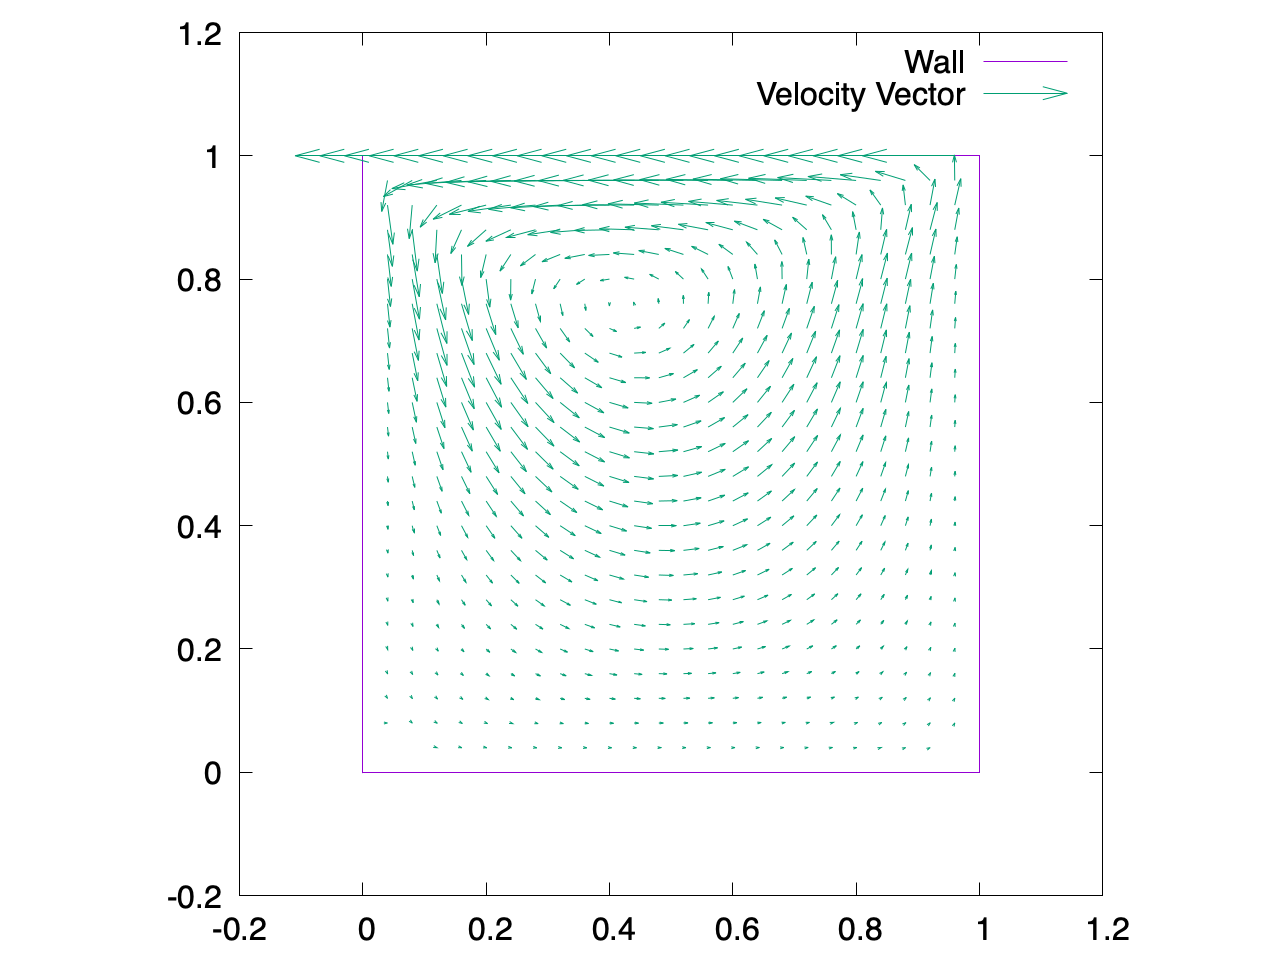
\includegraphics[height=9.5cm]{outputs/img/velocity_vector_re50.png}
  \caption{速度ベクトル図(i)}
  \label{fig:velocity_vector_re50}
\end{figure}
\begin{figure}[H]
  \centering
  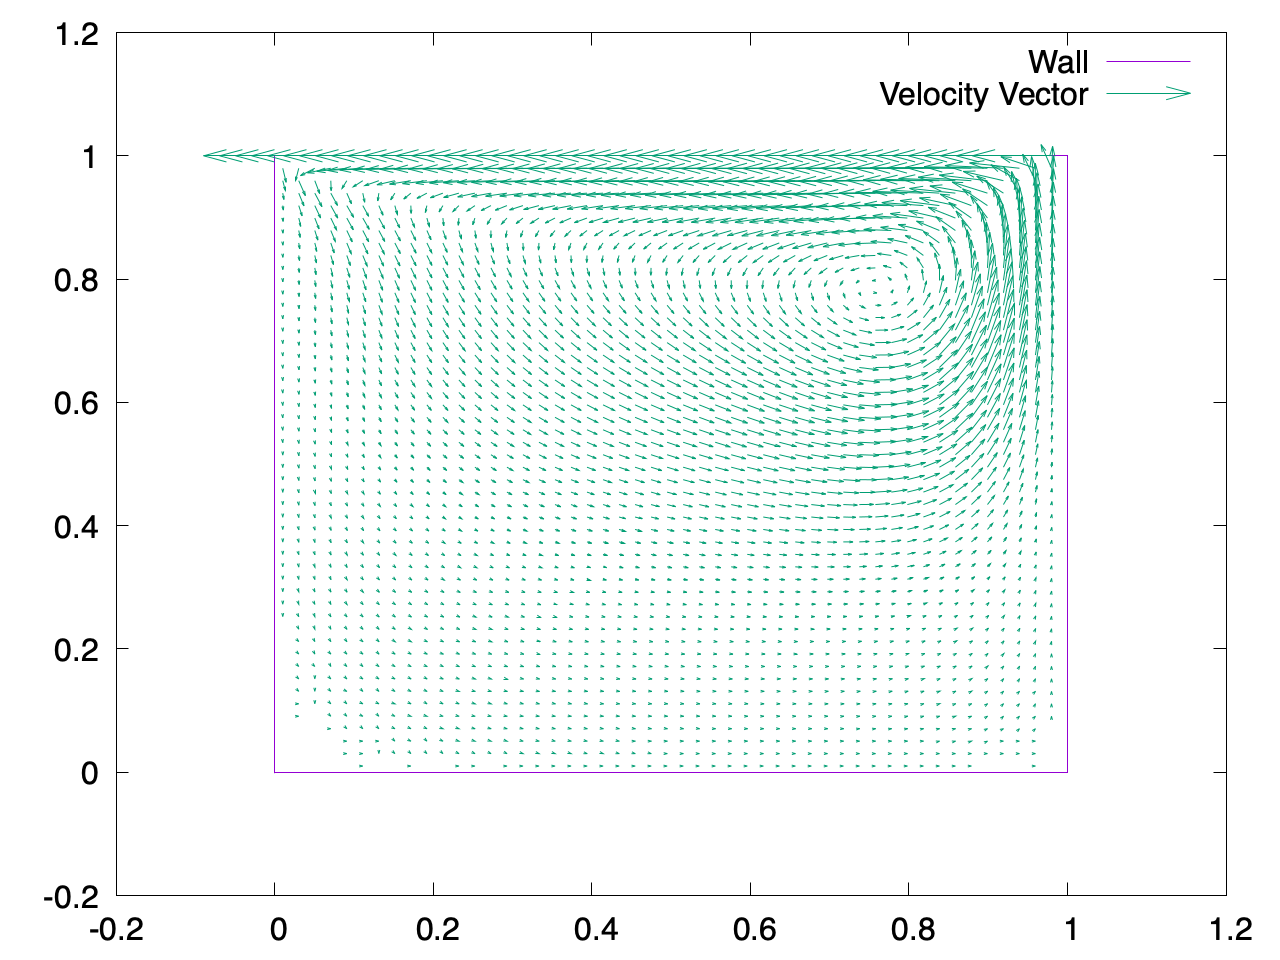
\includegraphics[height=9.5cm]{outputs/img/velocity_vector_re200.png}
  \caption{速度ベクトル図(ii)}
  \label{fig:velocity_vector_re200}
\end{figure}

また,速度ベクトルの向きを図3,4に示す.
点(0,0),(1,0)付近で時計回りの小さな渦が存在していることが確認できる.
時計回りの渦は点(0,0)付近のものの方が点(0,1)付近のものより大きく,点(0,0)付近の渦は条件(ii)の方が条件(i)より大きい.

\begin{figure}[H]
  \centering
  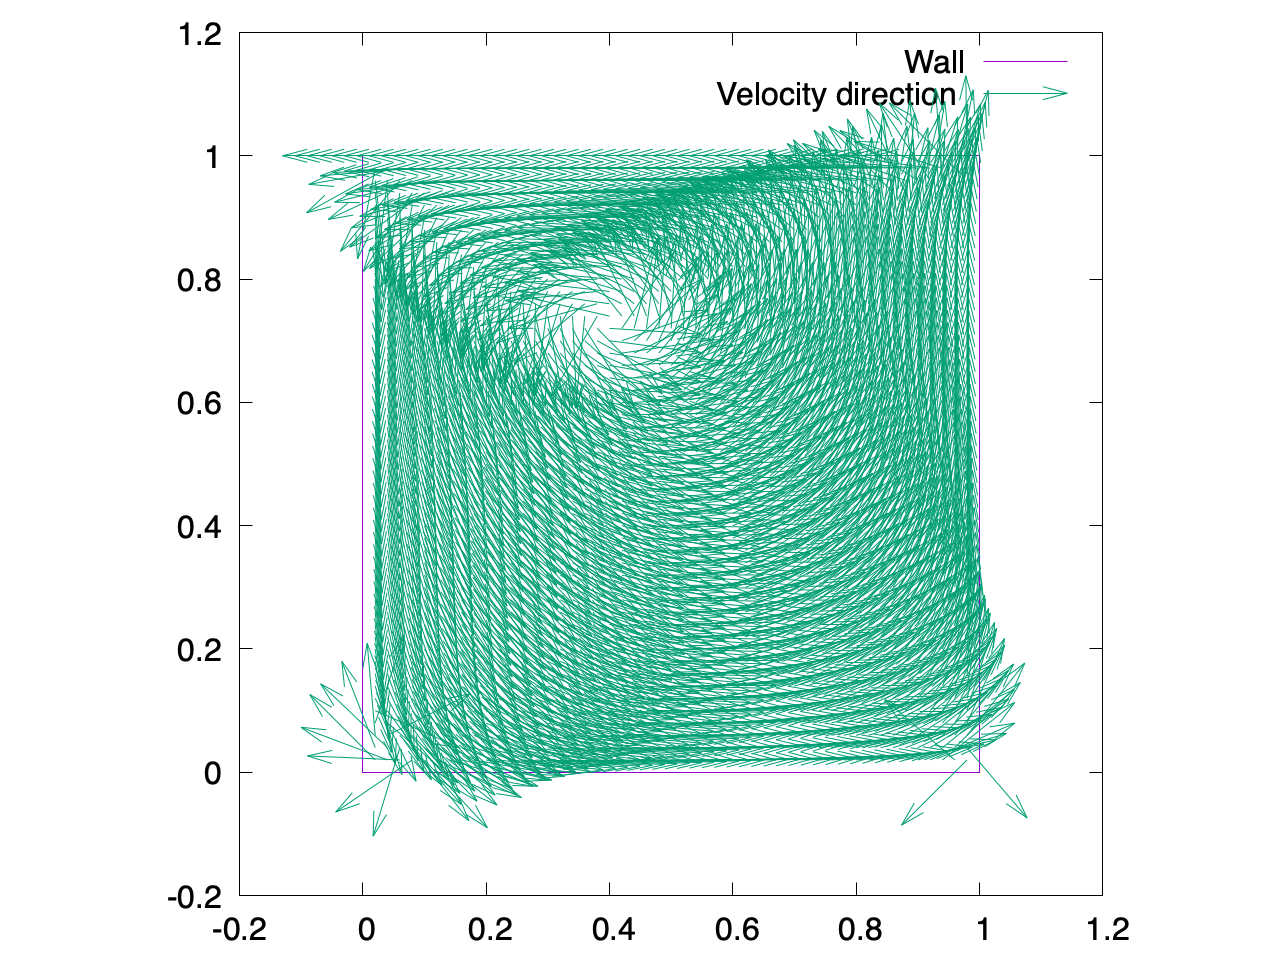
\includegraphics[height=9.5cm]{outputs/img/velocity_abs_re50.png}
  \caption{速度ベクトルの向き(i)}
\end{figure}
\begin{figure}[H]
  \centering
  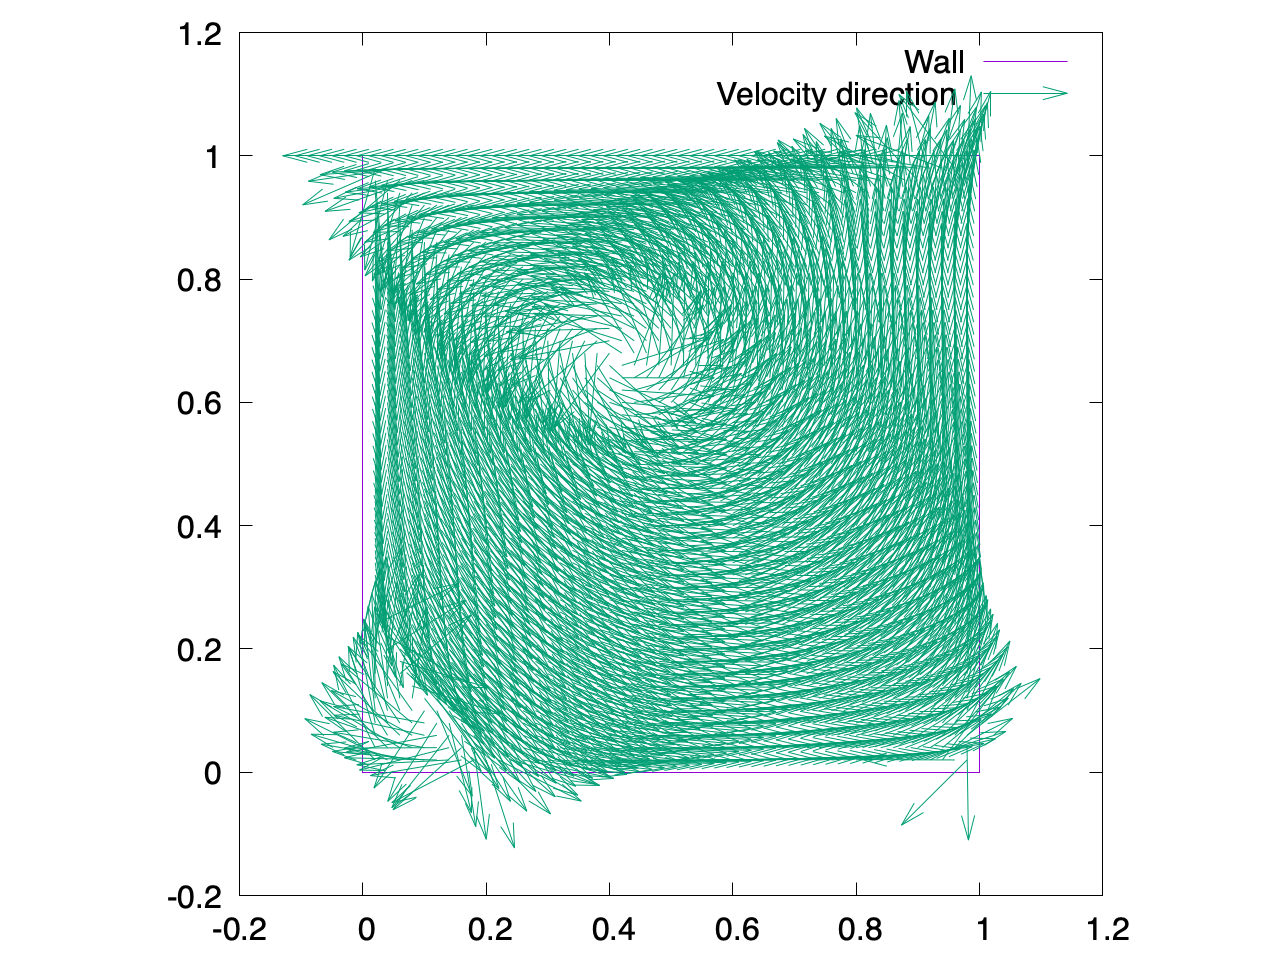
\includegraphics[height=9.5cm]{outputs/img/velocity_abs_re200.png}
  \caption{速度ベクトルの向き(ii)}
\end{figure}
\textcolor{red}{
底面付近の逆流渦を拡大した速度ベクトル図を図$5,6$に示す.
\begin{figure}[H]
  \begin{minipage}[c]{0.45\linewidth}
    \centering
    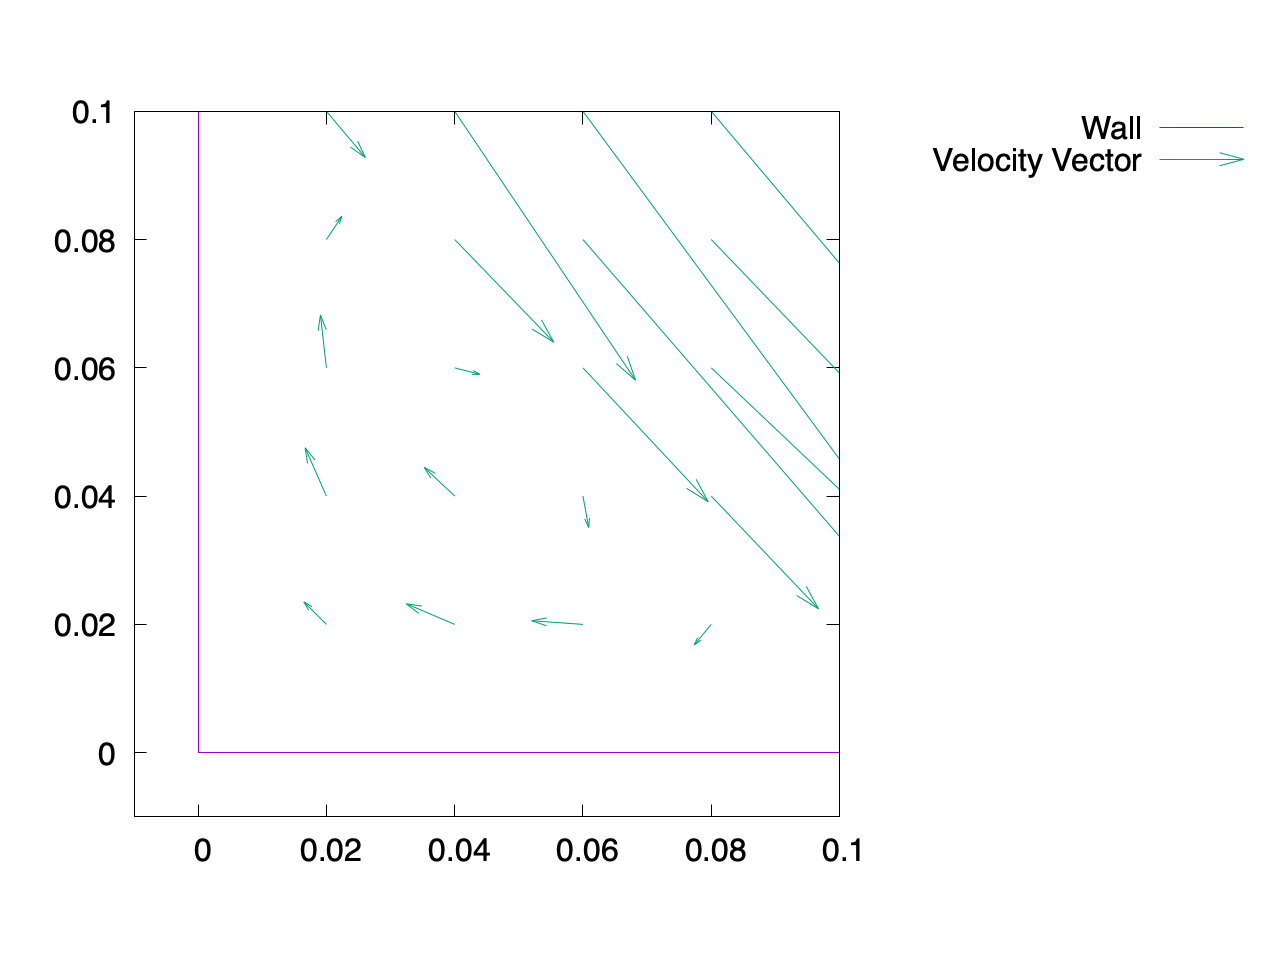
\includegraphics[height=7.5cm]{outputs/img/velocity_vector_corner1_re50.png}
    \subcaption{cavity左底部}\label{ラベル1}
  \end{minipage}
  \begin{minipage}[c]{0.45\linewidth}
    \centering
    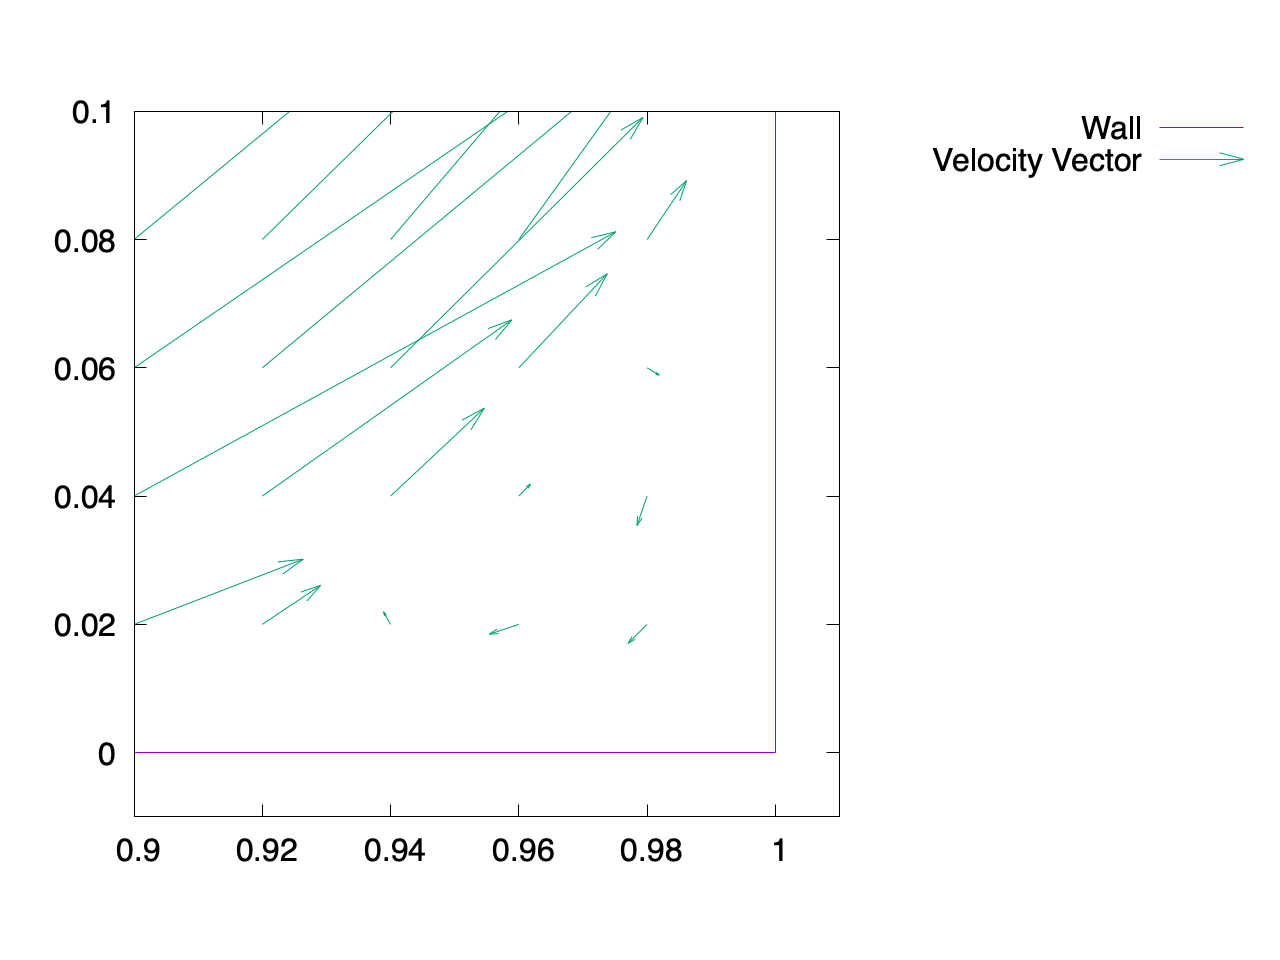
\includegraphics[height=7.5cm]{outputs/img/velocity_vector_corner2_re50.png}
    \subcaption{cavity右底部}\label{ラベル2}
  \end{minipage}
  \caption{拡大した速度ベクトル図(i)}\label{ラベル}
\end{figure}
\begin{figure}[H]
  \begin{minipage}[c]{0.45\linewidth}
    \centering
    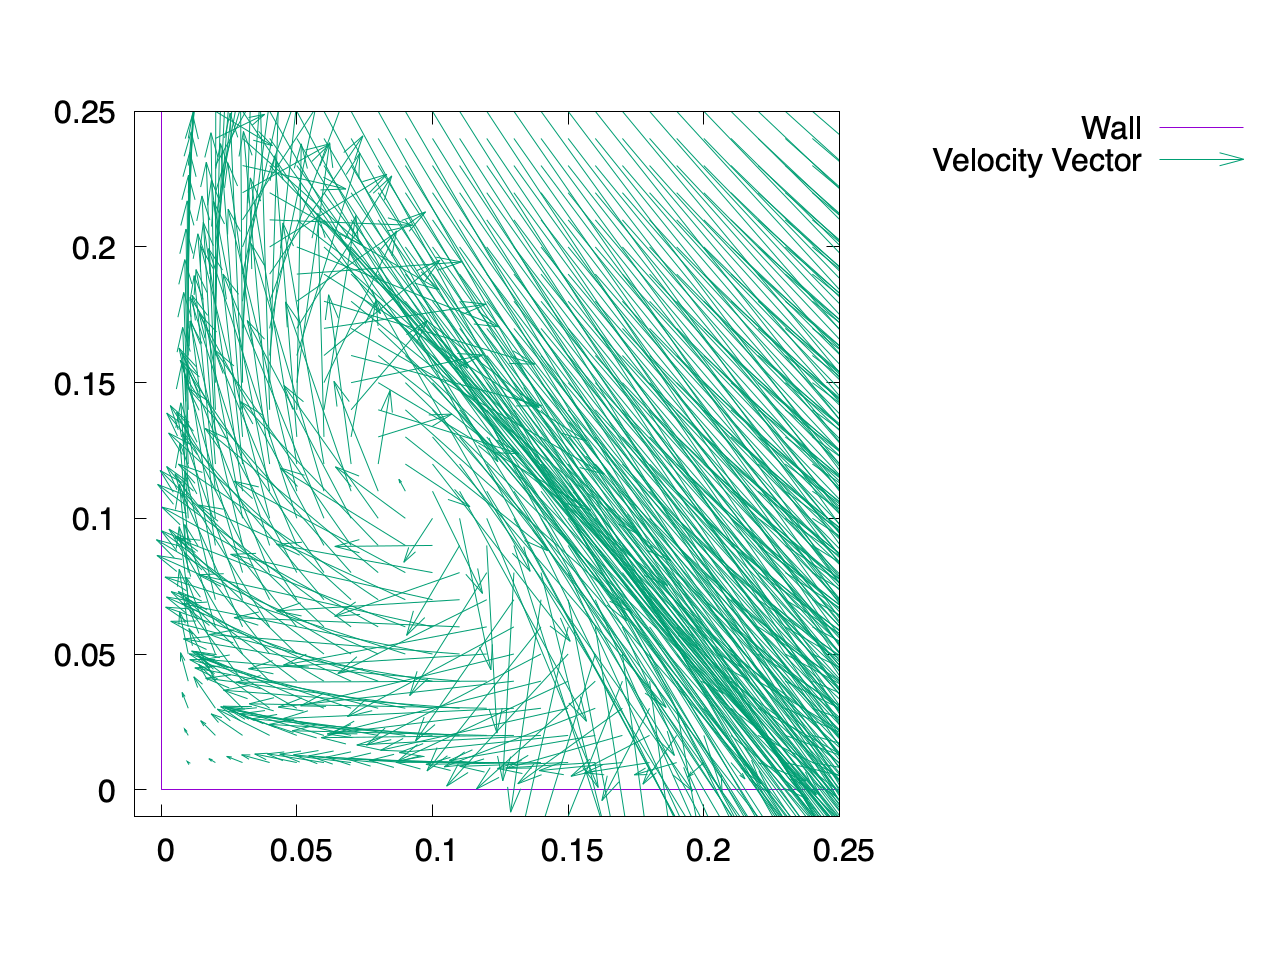
\includegraphics[height=7.5cm]{outputs/img/velocity_vector_corner1_re200.png}
    \subcaption{cavity左底部}\label{ラベル1}
  \end{minipage}
  \begin{minipage}[c]{0.45\linewidth}
    \centering
    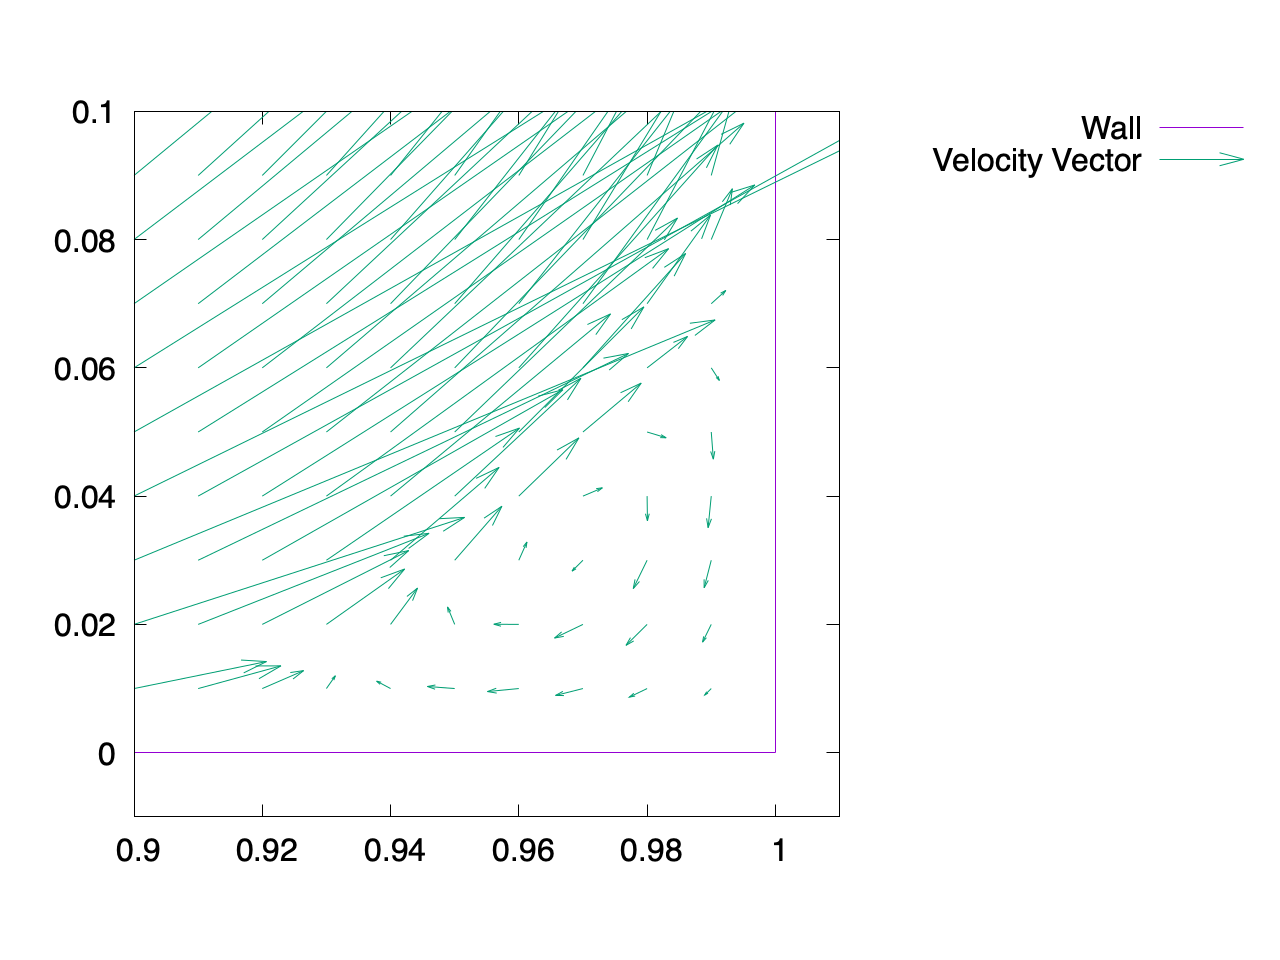
\includegraphics[height=7.5cm]{outputs/img/velocity_vector_corner2_re200.png}
    \subcaption{cavity右底部}\label{ラベル2}
  \end{minipage}
  \caption{拡大した速度ベクトル図(ii)}\label{ラベル}
\end{figure}
}


\subsection{流線図}

図7,8に今回得られた流線図を示す.

\begin{figure}[H]
  \centering
  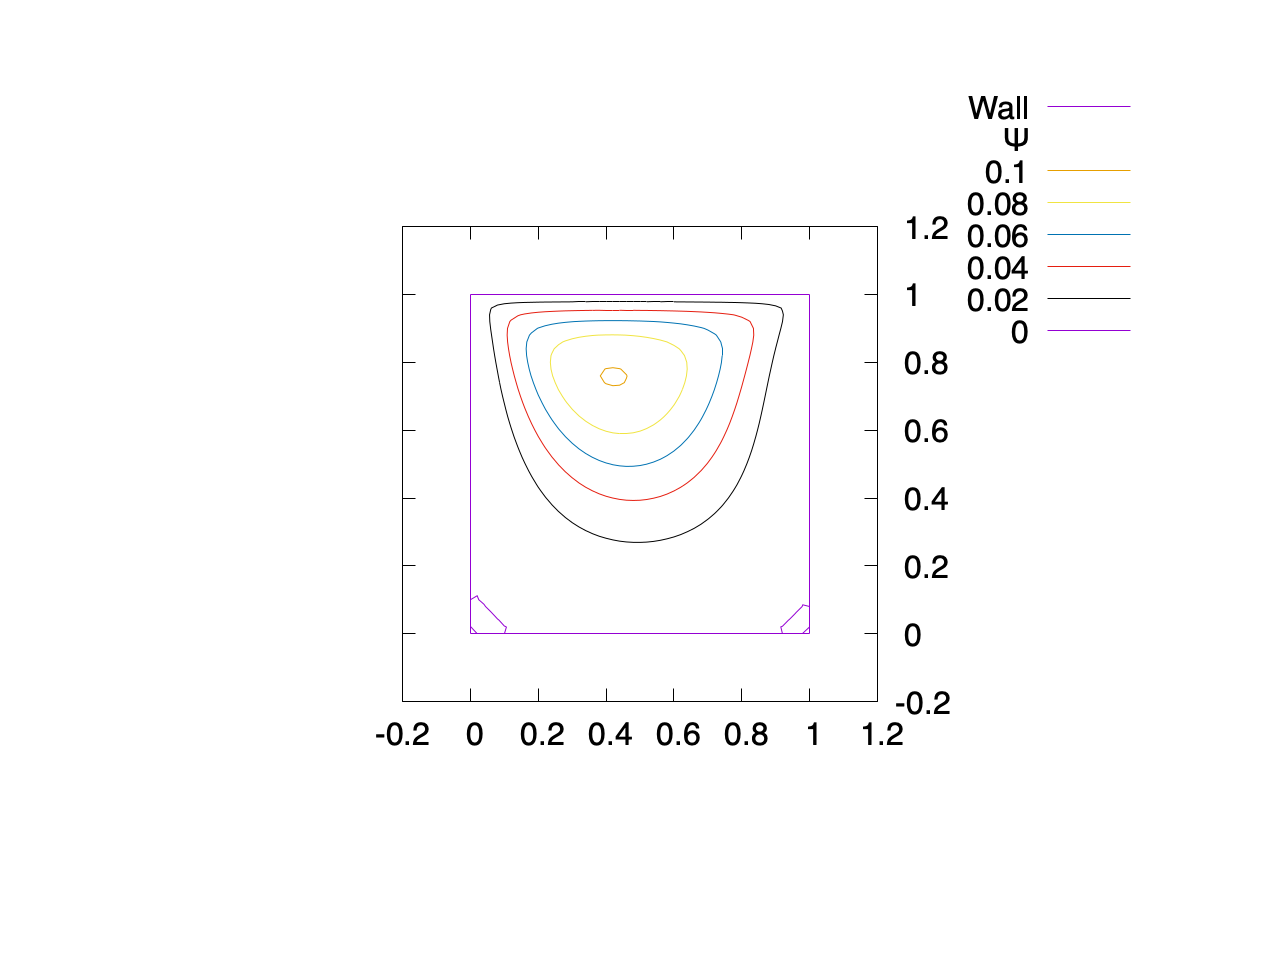
\includegraphics[height=9.5cm, clip, trim=0 200 0 0]{outputs/img/stream_line_re50.png}
  \caption{流線図(i)}
  \label{fig:velocity_vector_re50}
\end{figure}
\begin{figure}[H]
  \centering
  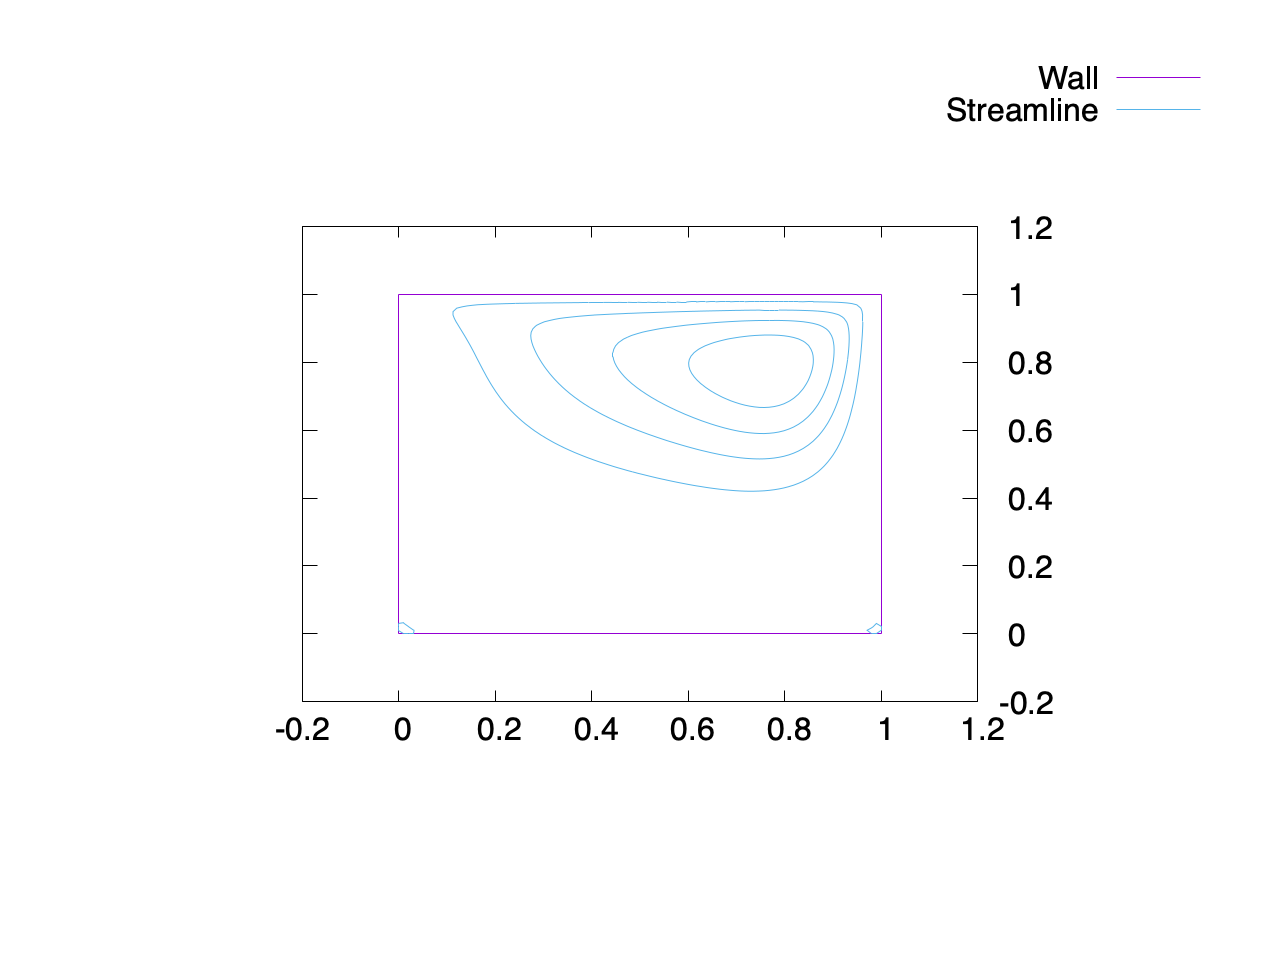
\includegraphics[height=9.5cm, clip, trim=0 200 0 0]{outputs/img/stream_line_re200.png}
  \caption{流線図(ii)}
  \label{fig:velocity_vector_re200}
\end{figure}
\textcolor{red}{
底面付近の逆流渦について拡大した流線図を図$9,10$に示す.ただし,流線間での流れ関数の差$\varDelta\psi$を底面付近の逆流渦内部で複数本引ける程度に小さくした時,
$\psi>0$の領域で流線が過密になり塗りつぶされてしまうため,$\psi\leq0$となる$\psi$について流線図を書いた.
\begin{figure}[H]
  \begin{minipage}[b]{0.50\linewidth}
    \centering
    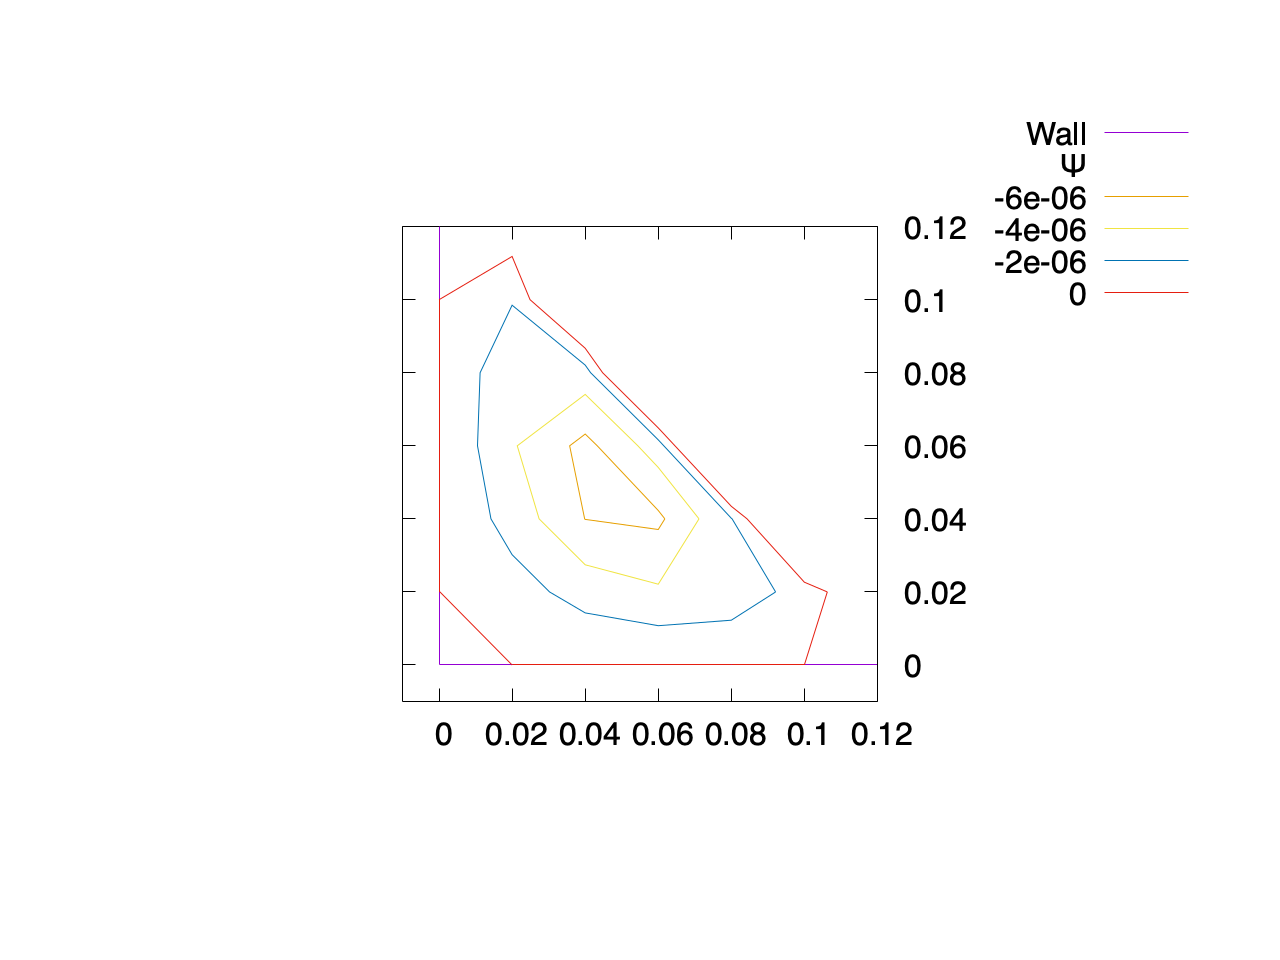
\includegraphics[height=7cm, clip, trim=300 150 100 50]{outputs/img/stream_line_corner1_re50.png}
    \subcaption{cavity左底部}\label{ラベル1}
  \end{minipage}
  \begin{minipage}[b]{0.50\linewidth}
    \centering
    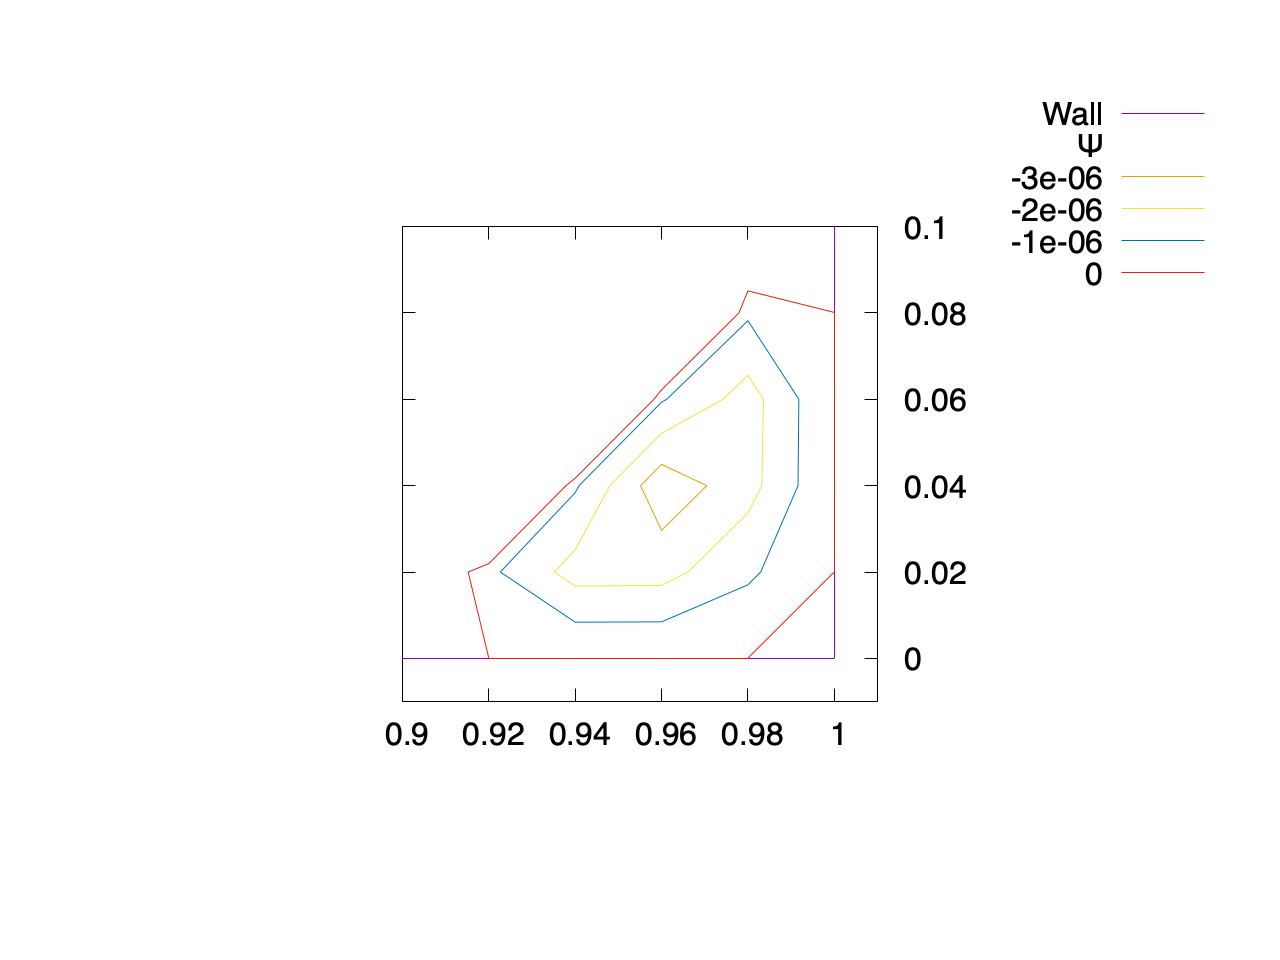
\includegraphics[height=7cm, clip, trim=300 150 100 50]{outputs/img/stream_line_corner2_re50.png}
    \subcaption{cavity右底部}\label{ラベル2}
  \end{minipage}
  \caption{拡大した流線図(i)}\label{ラベル}
\end{figure}
\begin{figure}[H]
  \begin{minipage}[c]{0.5\linewidth}
    \centering
    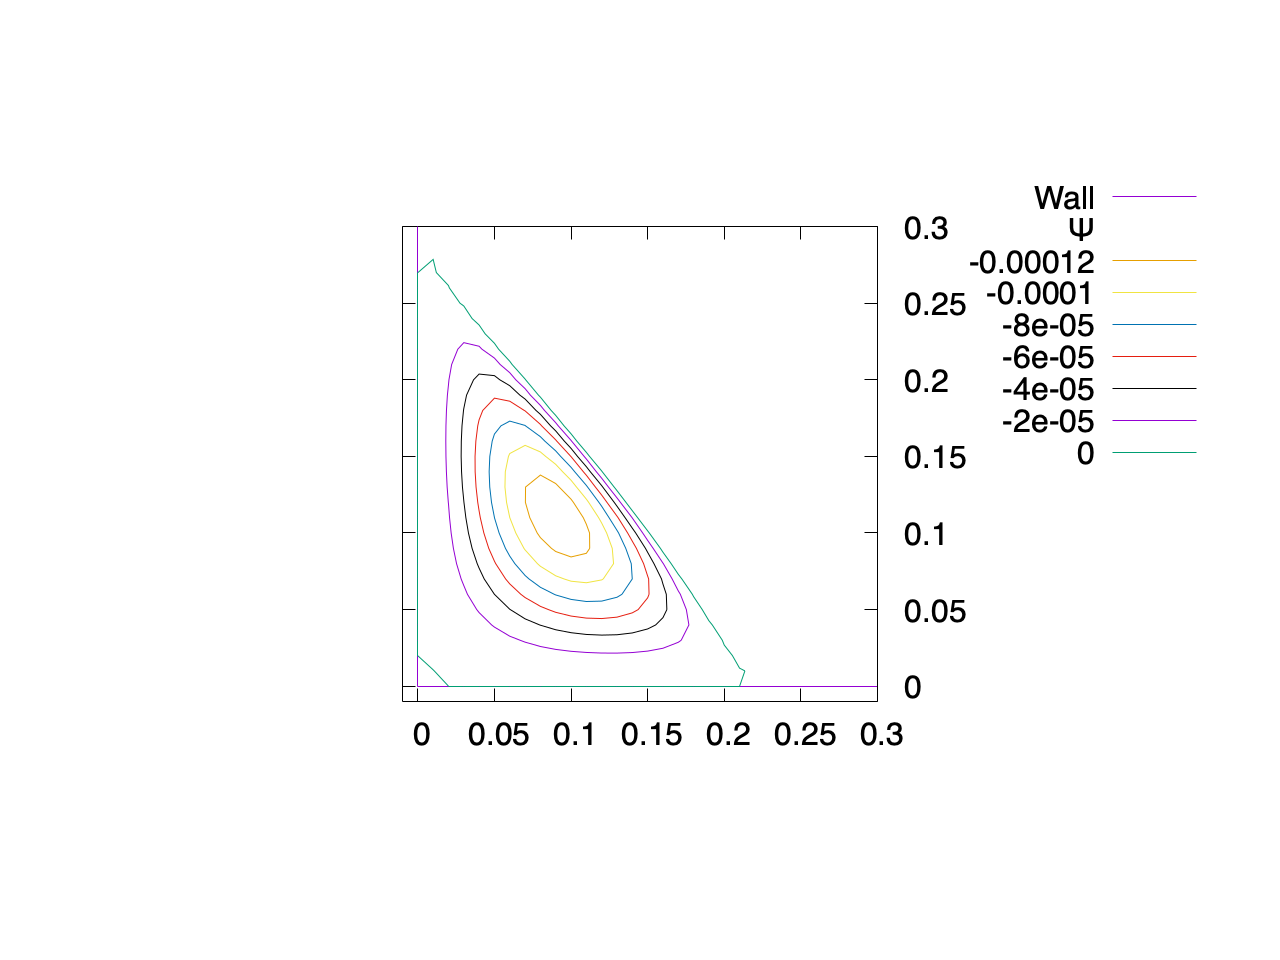
\includegraphics[height=7cm, clip, trim=300 150 100 50]{outputs/img/stream_line_corner1_re200.png}
    \subcaption{cavity左底部}\label{ラベル1}
  \end{minipage}
  \begin{minipage}[c]{0.5\linewidth}
    \centering
    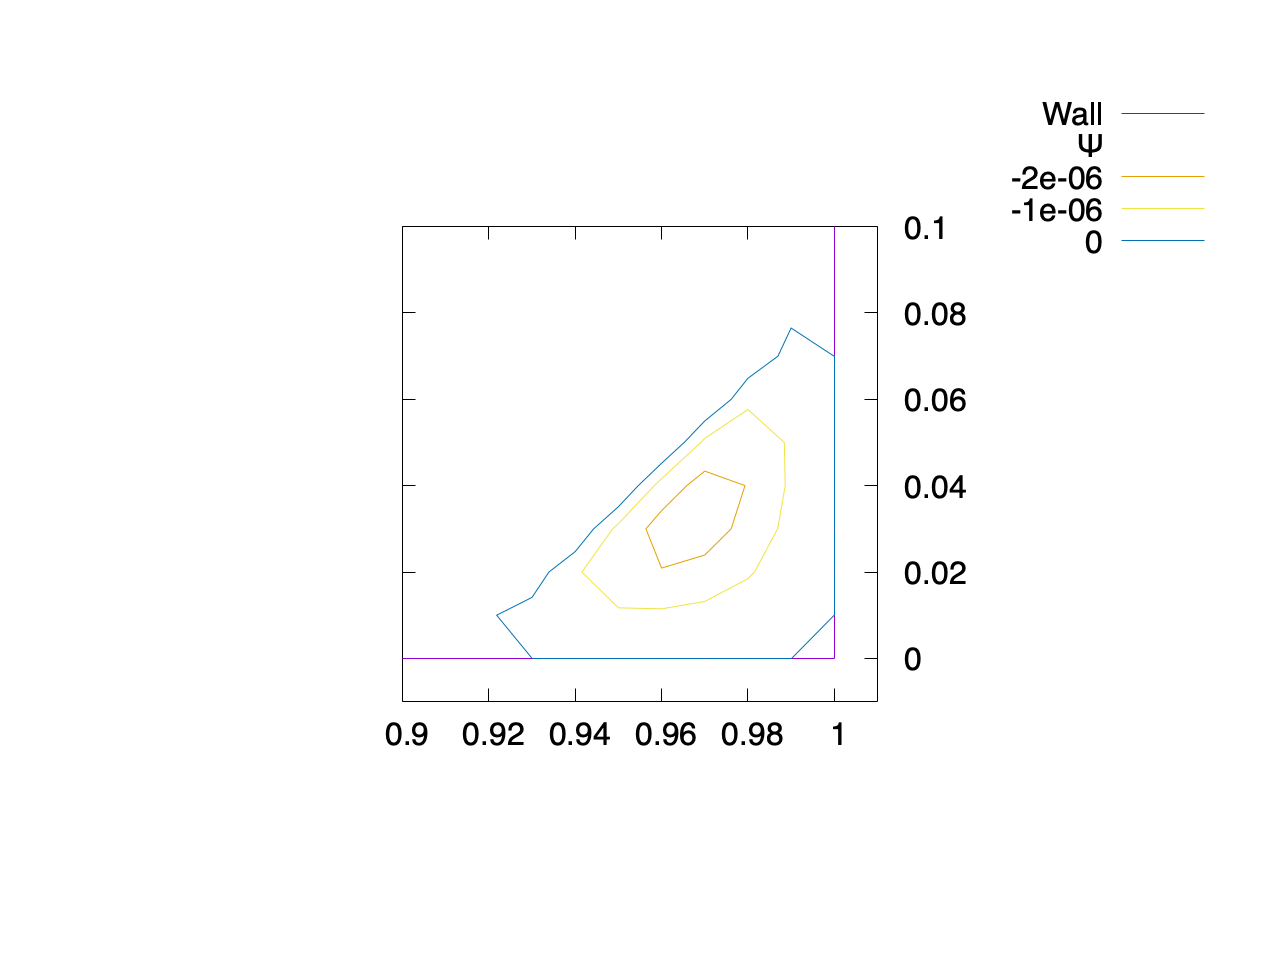
\includegraphics[height=7cm, clip, trim=300 150 100 50]{outputs/img/stream_line_corner2_re200.png}
    \subcaption{cavity右底部}\label{ラベル2}
  \end{minipage}
  \caption{拡大した流線図(ii)}\label{ラベル}
\end{figure}
}
\subsection{等圧線図}
図11,12に今回得られた等圧線図を示す.
条件(i), (ii)ともに点(0,1)付近で圧力が高く,点(1,1)付近で圧力が低くなった.
さらに,cavity上部中央付近でも圧力が基準圧より低い領域が見られた.

\begin{figure}[H]
  \centering
  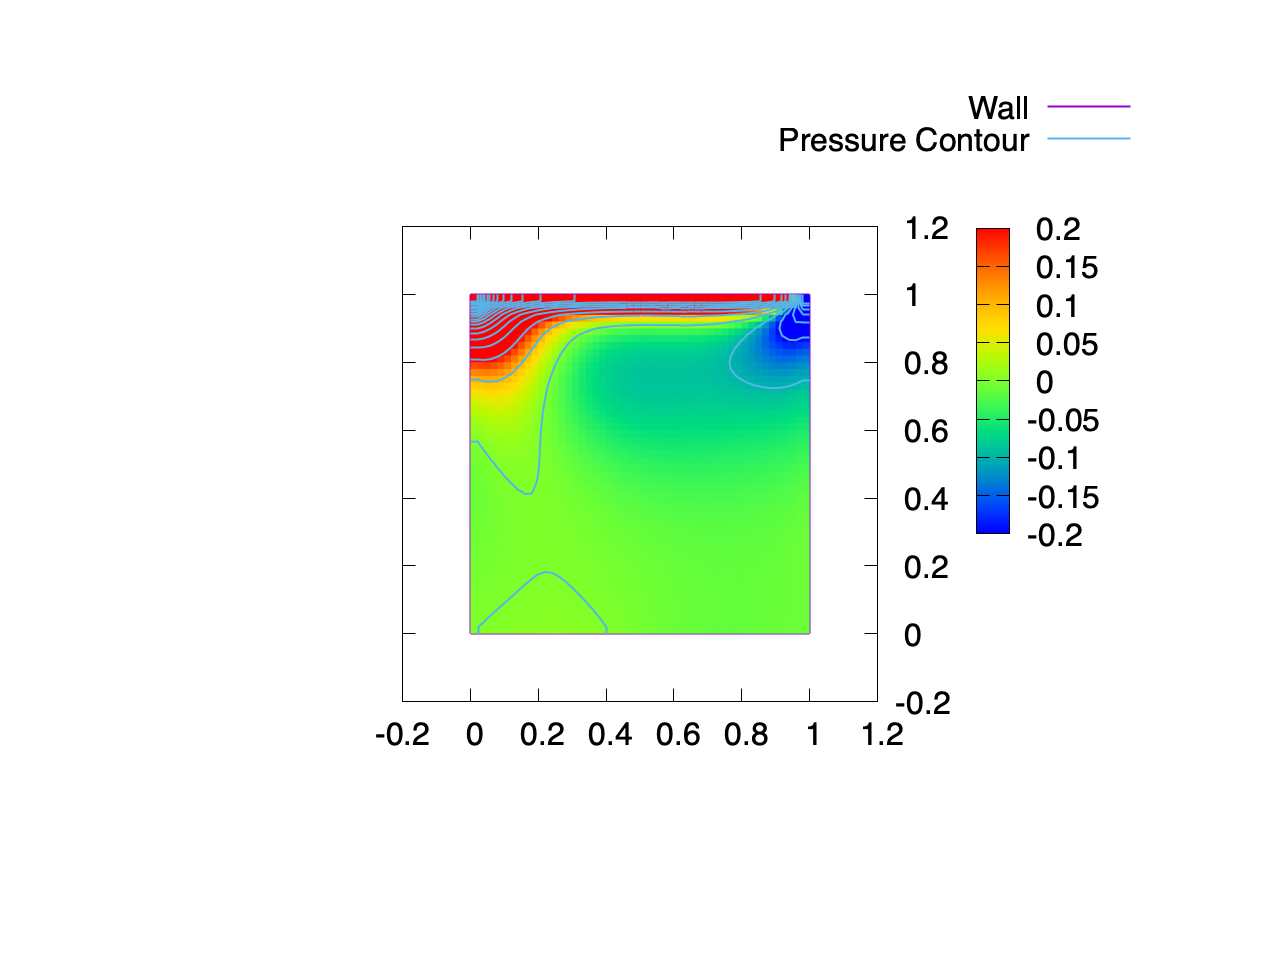
\includegraphics[height=9.5cm, clip, trim=0 200 0 0]{outputs/img/p_re50.png}
  \caption{等圧線図(i)}
  \label{fig:p_re50}
\end{figure}
\begin{figure}[H]
  \centering
  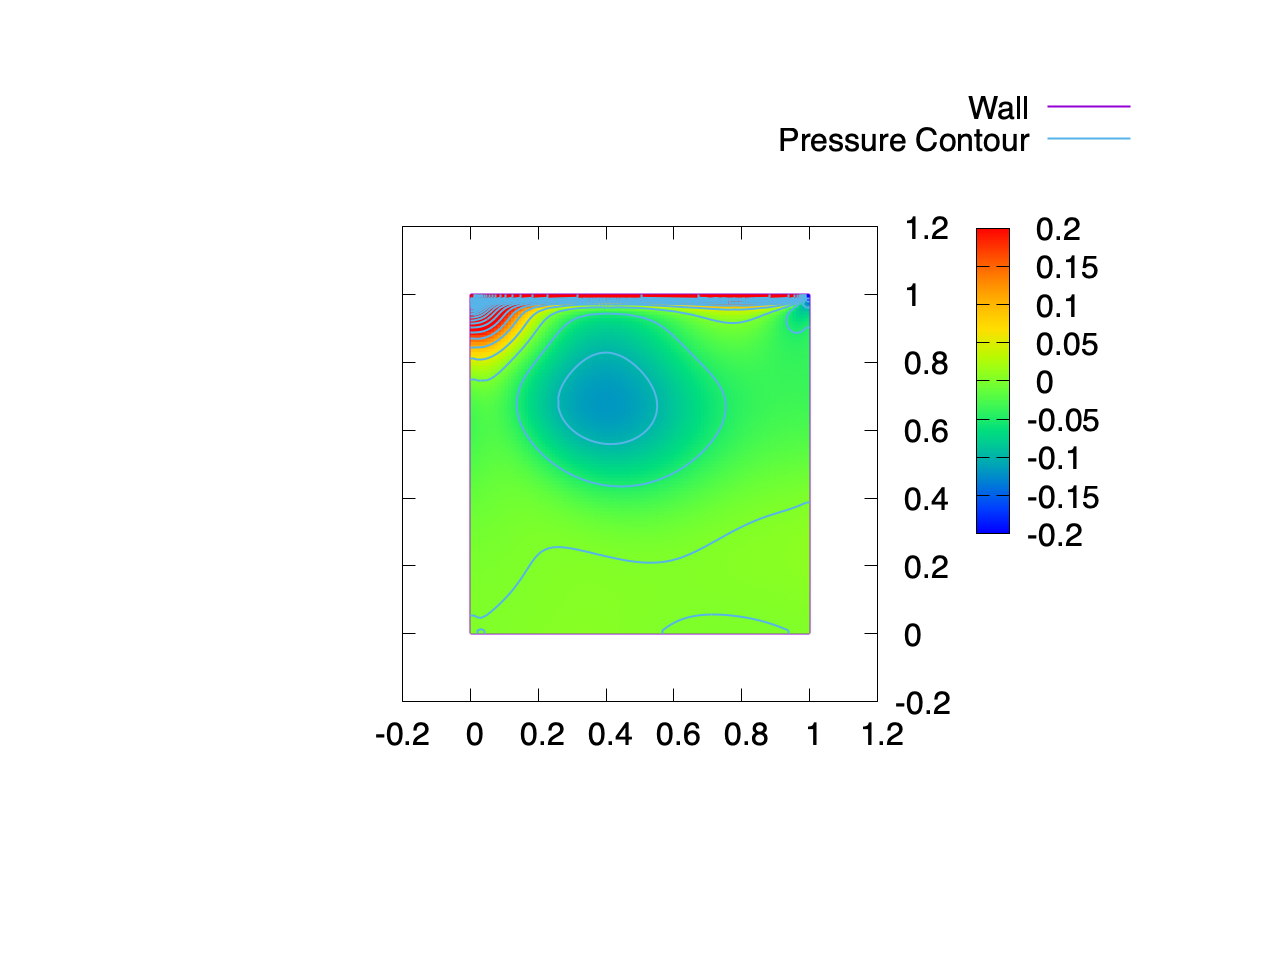
\includegraphics[height=9.5cm, clip,trim=0 200 0 0]{outputs/img/p_re200.png}
  \caption{等圧線図(ii)}
  \label{fig:p_re200}
\end{figure}

\begin{thebibliography}{9}
  %	\bibitem{1} \url{http://www.hal.t.u-tokyo.ac.jp/lab/ja/index_1.xhtml}
  %    \bibitem{2}Olga Russakovsky*, Jia Deng*, Hao Su, Jonathan Krause, Sanjeev Satheesh, Sean Ma, Zhiheng Huang, Andrej Karpathy, Aditya Khosla, Michael Bernstein, Alexander C. Berg and Li Fei-Fei. (* = equal contribution) ImageNet Large Scale Visual Recognition Challenge. IJCV, 2015.
  \bibitem{1} 研究室資料.流体の数値計算(川口光年先生1976年頃).pdf
  \bibitem{2} 越馬 遼 研究レポート (2021/6/17に提出されたもの)
\end{thebibliography}
\end{document}